\begin{frame}[plain]
  \Large
  \begin{columns}[c]
    \column{7cm}
    \begin{exampleblock}{}
      Database is looking good...
    \end{exampleblock}
    \column{4cm}
  \end{columns}
  \vspace{2cm}
  \begin{columns}[c]
    \column{3cm}
    \column{8cm}
    \begin{exampleblock}{}
      ... what about large computation?
    \end{exampleblock}
  \end{columns}
\end{frame}

\begin{frame}[plain]
  \Large
  \begin{columns}[c]
    \column{7cm}
    \begin{exampleblock}{}
      $\approx$ 2.5 billion galaxies in Bolshoi dataset,
      how many to process, on average, per request?
    \end{exampleblock}
    \column{4cm}
  \end{columns}
  \vspace{2cm}
  \begin{columns}[c]
    \column{3cm}
    \column{8cm}
    \begin{exampleblock}{}
      We will need to parallelise computation.
    \end{exampleblock}
  \end{columns}
\end{frame}

\begin{frame}[plain]
  \begin{block}{Science Modules}
    \vspace{1cm}
    \hspace{2cm}
    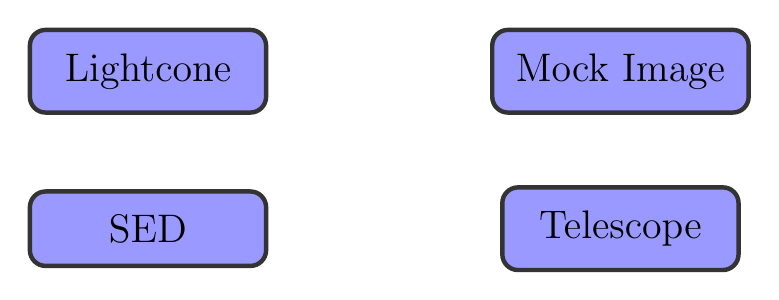
\begin{tikzpicture}[
        norm/.style={draw=black!80,rectangle,rounded corners=2mm,inner sep=3mm,fill=blue!40,ultra thick,minimum width=3cm}
      ]
      \node[norm] (lc) at (0,0) {{\Large Lightcone}};
      \node[norm] (sed) at (0,-2) {{\Large SED}};
      \node[norm] (mi) at (6,0) {{\Large Mock Image}};
      \node[norm] (te) at (6,-2) {{\Large Telescope}};
    \end{tikzpicture}
    \vspace{1cm}
  \end{block}
\end{frame}

\begin{frame}[plain]
  \begin{block}{Science Modules}
    \vspace{1cm}
    \hspace{2cm}
    \begin{tikzpicture}[
        norm/.style={draw=black!80,rectangle,rounded corners=2mm,inner sep=3mm,fill=blue!40,ultra thick,minimum width=3cm}
      ]
      \node[norm] (lc) at (0,0) {{\Large Lightcone}};
      \node[norm] (sed) at (0,-2) {{\Large SED}};
      \node[norm] (mi) at (6,0) {{\Large Mock Image}};
      \node[norm] (te) at (6,-2) {{\Large Telescope}};
      % Connections.
      \draw[-triangle 90] (lc) -- (sed);
      \draw[-triangle 90] (sed) -- (mi);
      \draw[-triangle 90] (mi) -- (te);
    \end{tikzpicture}
    \vspace{1cm}
  \end{block}
\end{frame}

\begin{frame}[plain]
  \begin{center}
  \begin{tikzpicture}
    \path[use as bounding box] (0,-1) rectangle (10,7);
    % Border.
    \draw (0,0) rectangle (6,6);
    % Objects.
    \pgfmathsetseed{1187}
    \foreach \x in {1,...,100}
    \fill[black!50] ($ (0,0) + 6*(rnd,rnd) $) circle(1pt);
    % Cone.
    \filldraw[fill=blue,fill opacity=0.1,draw=blue!90] (0,0) -- (5,3) arc (30.96:59.04:5.83) -- cycle;
    % Redshift arcs.
    \begin{scope}
      \clip (0,-1) rectangle(6,6);
      \foreach \x/\z in {1.4/0, 2.8/1, 4.2/2, 5.6/3, 7/4}
        \draw[black!75,dashed] (\x,0) node[anchor=north]{$z_\z$} arc (0:90:\x);
    \end{scope}
  \end{tikzpicture}
  \end{center}
\end{frame}

\begin{frame}[plain]
  \begin{center}
  \begin{tikzpicture}
    \path[use as bounding box] (0,-1) rectangle (10,7);
    % Border.
    \draw (0,0) rectangle (6,6);
    % Objects.
    \pgfmathsetseed{1187}
    \foreach \x in {1,...,100}
    \fill[black!50] ($ (0,0) + 6*(rnd,rnd) $) circle(1pt);
    % Cone.
    \filldraw[fill=blue,fill opacity=0.1,draw=blue!90] (0,0) -- (5,3) arc (30.96:59.04:5.83) -- cycle;
   \draw[blue!90] (0,0) -- (4.45,3.77);
   \draw[blue!90] (0,0) -- (3.77,4.45);
   \draw (2.9,4) node{$P_0$};
   \draw (3.5,3.5) node{$P_1$};
   \draw (4,2.9) node{$P_2$};
    % Redshift arcs.
    \begin{scope}
      \clip (0,-1) rectangle(6,6);
      \foreach \x/\z in {1.4/0, 2.8/1, 4.2/2, 5.6/3, 7/4}
        \draw[black!75,dashed] (\x,0) node[anchor=north]{$z_\z$} arc (0:90:\x);
    \end{scope}
  \end{tikzpicture}
  \end{center}
\end{frame}

\begin{frame}[plain]
  \begin{center}
  \begin{tikzpicture}
    \path[use as bounding box] (0,-1) rectangle (10,7);
    % Border.
    \draw (0,0) rectangle (6,6);
    % Objects.
    \pgfmathsetseed{1187}
    \foreach \x in {1,...,100}
    \fill[black!50] ($ (0,0) + 6*(rnd,rnd) $) circle(1pt);
    % Cone.
    \filldraw[fill=blue,fill opacity=0.1,draw=blue!90] (0,0) -- (5,3) arc (30.96:59.04:5.83) -- cycle;
   \draw[blue!90] (0,0) -- (4.45,3.77);
   \draw[blue!90] (0,0) -- (3.77,4.45);
   \draw (2.9,4) node{$P_0$};
   \draw (3.5,3.5) node{$P_1$};
   \draw (4,2.9) node{$P_2$};
    % Redshift arcs.
    \begin{scope}
      \clip (0,-1) rectangle(6,6);
      \foreach \x/\z in {1.4/0, 2.8/1, 4.2/2, 5.6/3, 7/4}
        \draw[black!75,dashed] (\x,0) node[anchor=north]{$z_\z$} arc (0:90:\x);
    \end{scope}
    % Text.
    \node at (8.5,4) {Balanced? Probably, but};
    \node at (8.5,3.3) {need to investigate.};
  \end{tikzpicture}
  \end{center}
\end{frame}

\begin{frame}[plain]
  \Large
  \begin{columns}[c]
    \column{7cm}
    \begin{exampleblock}{}
      We will also utilise GPUs (eventually).
    \end{exampleblock}
    \column{4cm}
  \end{columns}
  \vspace{2cm}
  \begin{columns}[c]
    \column{3cm}
    \column{8cm}
    \begin{block}{Algorithms}
      \begin{itemize}
        \item Cubic spline interpolation.
        \item Fourth order Gaussian integration.
        \item Both easily accelerated by GPUs.
      \end{itemize}
    \end{block}
  \end{columns}
\end{frame}
